\documentclass[final]{beamer}
\usetheme{RJH}
\usepackage[orientation=landscape,size=a0,scale=2.0]{beamerposter}
\usepackage[absolute,overlay]{textpos}
\usepackage[english]{babel}
\usepackage{color}
\setlength{\TPHorizModule}{1cm}
\setlength{\TPVertModule}{1cm}

\usepackage{lmodern}% http://ctan.org/pkg/lm

\title{Parallel Metropolis-Hastings Algorithm by Prefetching}
\author{Boyan Bejanov (bbejanov@bankofcanada.ca) }
\footer{
\parbox{0.48\textwidth}{
    \flushleft \small
    Data Day, 24 April 2014, Carleton University
    }
\hfill
\parbox{0.48\textwidth}{\flushright
Bank of Canada}
}
\date{April 2014}

\newcounter{SlideNO}
\newcommand\slide{\stepcounter{SlideNO}\theSlideNO.~} 

\begin{document}
\begin{frame}[t]{} 

\begin{columns}[t]
    \begin{column}{0.3\textwidth}

        \begin{block}{\slide Introduction}
            \begin{description}
             \item[Metropolis-Hastings (MH)] is a Markov Chain Monte Carlo (MCMC)
                algorithm which is used to simulate random samples from
                probability distributions that are difficult to simulate
                otherwise.                
            \item[Prefetching] is a parallelization technique for the
                MH algorithm.  It is applicable in situations
                where the target p.d.f.,
                \textbf{ $\boldsymbol{\pi}\mathbf{(x)}$, is
                    \begin{itemize}
                        \item computationally very expensive;
                        \item impractical to parallelize.                
                    \end{itemize}
                }
            \end{description}
            E.g. Bayesian inference for  economic models.
        \end{block}
       
        \begin{block}{\slide MH algorithm}
            Markov chain with accept-reject transition rule:
            \begin{itemize}
                \item Current state is $X_0$.
                \item Propose candidate $Y \sim q(X_0, \cdot)$.
                \item Accept the candidate with probability
                    $$\alpha = \frac{\pi(Y)q(Y,X_0)}{\pi(X_0)q(X_0,Y)}.$$
            \end{itemize}
        \end{block}

        \begin{block}{\slide Prefetching tree}
            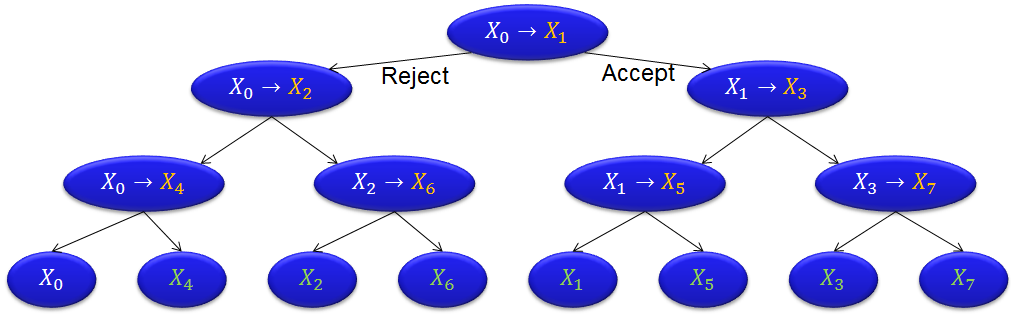
\includegraphics[width=.9\textwidth]{PrefetchingTree.png}
            \begin{itemize}
            \item At each node the current state is in white.
            \item The proposed candidate is in orange.
            \end{itemize}
        \end{block}
     
    \end{column}
    \begin{column}{0.3\textwidth}

        \begin{block}{\slide Implemetation}        
        \centering {\small
        \begin{tabular}{|l|c||c||c|c||c|c|c|c||c|c|c|c|c|c|c|c|}
            \hline
            step $s$ & 0 & 1 & \multicolumn{2}{c||}{2} & \multicolumn{4}{c||}{3} & \multicolumn{8}{c|}{4} \\
            \hline
            current $c$ & $\ast$ & 0 & 0 & 1 & 0 & 1 & 2 & 3 & 0 & 1 & 2 & 3 & 4 & 5 & 6 & 7 \\
            \hline
            proposed $k$ & 0 & 1 & 2 & 3 & 4 & 5 & 6 & 7 & 8 & 9 & 10 & 11 & 12 & 13 & 14 & 15\\
            \hline
        \end{tabular}
        }
        \begin{itemize}
            \item $X_k$ was proposed at step $s=\left\lfloor\log k\right\rfloor+1$.
            \item $X_k$ was proposed from $X_c$, $c=k-2^{s-1}$.
            \item The two children of proposal $X_k$ are $X_a$ and $X_r,$ where
                $a = k+2^s$ and $r = a-2^{s-1}$.
        \end{itemize}
        \end{block}

        \begin{block}{\slide Full prefetching}
            \begin{itemize}
            \item Consider all $2^n$ possible paths $n$ steps ahead.
            \item Compute $2^n-1$ evaluations of $\pi(\cdot)$ in parallel.
            \item Run $n$ steps of the Markov chain sequentially.
            \end{itemize}
            
        \end{block}

        \begin{block}{\slide Complexity of full prefetching}
            \begin{description}
                \item[Sequential time] $\displaystyle T_s = n$
                \item[Parallel time] $\displaystyle T(n,p) = \frac{2^n-1}{p}$
                \item[Speedup] $\displaystyle s(n,p) = \frac{np}{2^n-1}$
                \item[N.B.] \textit{\textcolor{red}{Speedup  is not logarithmic in $p$.}}
            \end{description}
        \end{block}

        \begin{block}{\slide Speedup graph: full prefetching}
        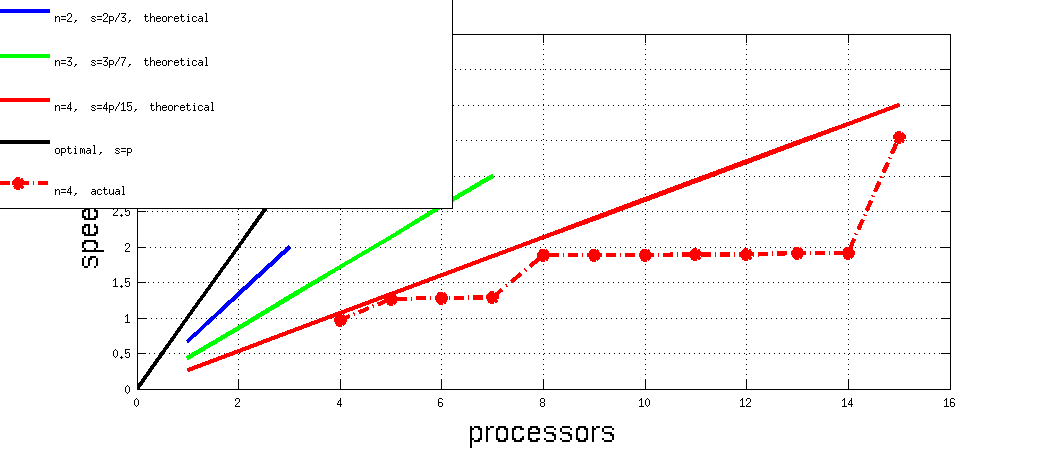
\includegraphics[width=1\textwidth]{speedup-full.png}
        \end{block}
      
    \end{column}
    \begin{column}{0.3\textwidth}

       \begin{block}{\slide Incomplete prefetching}
            \begin{itemize}
            \item Prefetch only $p$ proposals, not the full tree.
            %~ \item For $p<2^n-1$ the chain may not make $n$ steps
            \item By scaling the proposal distribution, $q(x,y)$, we can 
                control the acceptance rate, denoted $\alpha^*$.
            %~ \item At each branch the probability to accept is $\alpha^*$ and
                %~ the probability to reject is $1-\alpha^*$.
            %~ \item The probability to reach given candidate is the product
                %~ of all probabilities along its path.
            \item Choose the $p$ candidates to maximize the expected
                depth to be reached, denoted $D(p)$.
            \end{itemize}
        \end{block}

        \begin{block}{\slide Complexity of incomplete prefetching}
            \begin{description}
                \item[Parallel time] $ T(p) = \frac{n}{D(p)}$
                \item[Speedup] $ s(p) = D(p) \phantom{\frac{M}{M}}$
            \end{description}
            %~ \vspace{2ex}
            %~ \begin{itemize}
                %~ \item E.g. for $\alpha^* = 0.234$
            %~ \end{itemize}
            %~ \centerline{\small
            %~ \begin{tabular}{|c|c|c|c|c|c|c|c|c|c|c|} % c|c|c|c|c|}
                %~ \hline
                %~ processors $p$    &2    &3     &4     &5     &6     &7     &8     &9   \\%  &10     &11    &12   &13   &14    & 15 \\
                %~ \hline
                %~ $D(p)$ &1.77 & 2.35 & 2.80 & 3.15 & 3.41 & 3.64 & 3.84 & 4.03 \\%& 4.20  & 4.36 &4.49 &4.63 & 4.77 & 4.88  \\
                %~ \hline
            %~ \end{tabular}
            %~ }
        \end{block}

        \begin{block}{\slide Speedup graph: incomplete}
        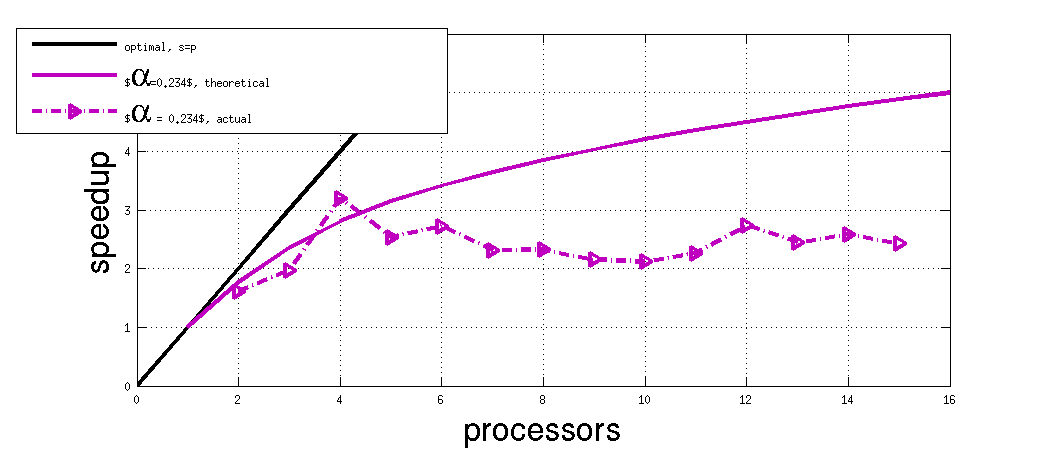
\includegraphics[width=1\textwidth]{speedup-partial.png}
        \end{block}

        \begin{block}{\slide Caveat emptor}
            \begin{itemize}
                \item Full prefetching provides speedup at the cost of
                    exponential number of processors $\Rightarrow$ inefficient.
                \item Incomplete prefetching gives improved \textit{expected}
                    efficiency, although not guaranteed.
            \end{itemize}
        \end{block}

        \begin{block}{\slide References}
            \begin{itemize}\small {
                \item A.E.~Brockwell, \textit{JCGS}, 2006, 15(1), 246-261.
                \item J.~Byrd, S.~Jarvis, A.H.~Bhalerao, \textit{ISPDP}, 2008, 1-8.         
                \item I.~Strid, \textit{CSDA}, 2010, 54(11), 2814-2835.
            } \end{itemize}
        \end{block}
        
      
    \end{column}
\end{columns}

\end{frame}
\end{document}
